% !TEX TS-program = pdflatex
% RESIDENTIAL_SITE_DESIGN.tex
% Re-siting of the reference design to a residential rooftop in the
% New Administrative Capital. Numbers produced by
% scripts/nac_residential_design.py (NASA POWER hourly, NAC point, 2025)
% and archived in output/nac_tec_robot_results.json. Benban outputs are
% untouched and remain the feasibility-evidence climate.
% NOTE: colortbl deliberately avoided (MiKTeX colortbl/array incompatibility).
\documentclass[11pt,a4paper]{article}

\usepackage[margin=2.2cm]{geometry}
\usepackage[T1]{fontenc}
\usepackage[utf8]{inputenc}
\usepackage{lmodern}
\usepackage{microtype}
\usepackage{amsmath,amssymb}
\usepackage{booktabs}
\usepackage{array}
\usepackage{graphicx}
\usepackage{siunitx}
\sisetup{group-separator={,},group-minimum-digits=4,per-mode=symbol,
         range-units=single,detect-all}
\DeclareSIUnit{\Wp}{Wp}
\DeclareSIUnit{\kWp}{kWp}
\DeclareSIUnit{\dy}{d}
\DeclareSIUnit{\yr}{yr}
\usepackage{enumitem}
\usepackage[hidelinks]{hyperref}
\usepackage{titlesec}
\titleformat{\section}{\large\bfseries}{\thesection.}{0.5em}{}
\titleformat{\subsection}{\normalsize\bfseries}{\thesubsection}{0.5em}{}
\emergencystretch=1.5em

\title{\textbf{Residential Reference Deployment}\\[0.4em]
\large Autonomous Thermoelectric Atmospheric-Water PV-Cleaning Robot\\[0.2em]
\normalsize Re-siting of the design basis to a rooftop array in the
New Administrative Capital, Egypt}
\author{Rahma El-Hamouly, Graduation Project (REE598)}
\date{12 June 2026}

\begin{document}
\maketitle

\begin{abstract}
\noindent
The frozen design package sized the robot against Benban (Aswan) 2020
climate, where full water self-sufficiency for a single \SI{2}{\metre\squared}
panel already needed 69 TEC tiles and \SI{5.32}{\kilo\watt\hour} per day.
This document moves the reference deployment to a \SI{9.9}{\kWp} residential
rooftop in the New Administrative Capital (NAC) and reruns the same
simulation engine on NASA POWER hourly data for 2025 at the NAC point
\cite{nasa_power_nac2025}. The climate change is decisive: per-tile yield
rises from \SI{5.35}{\liter\per\yr} at Benban to \SI{38.7}{\liter\per\yr}
at NAC, a factor of 7.2, with no dead summer months. The microfibre brush
cleans at \SI{0.3}{\liter\per\metre\squared}, so washing
\SI{46}{\metre\squared} of glass every \num{3.5} days consumes only
\SI{1.44}{\cubic\metre\per\yr}, and full atmospheric self-supply is feasible:
38 TEC tiles drawing \SI{6.47}{\kilo\watt\hour\per\dy}, about
\SI{14}{\percent} of what the array itself generates (19 tiles and
\SI{7}{\percent} on a weekly schedule). The recommended design therefore
sizes the dockside AWG for \SI{100}{\percent} self-supply: 38 tiles,
\SI{38.7}{\liter\per\yr} per tile, with a \SI{300}{\liter} storage tank to
bridge seasonal swings.
The robot itself is mechanically unchanged; the \ang{26} tilt raises
traction torque by \SI{5}{\percent} and stays inside the selected motor's
continuous band. A standalone off-grid dock with its own dedicated PV and
battery prices at \num{224756}~EGP for the 100\,\% case, but that figure is
dominated by the dedicated supply hardware. Since the house already carries
a \SI{9.9}{\kWp} array, the dock can draw its night load from the house bus,
and the marginal AWG hardware (38 tiles plus heat sinks, fans, cold plate,
and switching) is only about \num{14000}~EGP. Benban remains in the thesis
as feasibility evidence; NAC becomes the reference deployment case.
\end{abstract}

% =============================================================================
\section{Scope}
% =============================================================================

The project pivot of April 2026 fixed three deployment scales for the robot,
with residential rooftops in Egypt's new cities as the second scale and the
new-cities programme as the deployment intent \cite{egypt2030vision}. All
quantitative design work so far, however, sits on the Benban hourly climate
of 2020. This document does one thing: it re-sites the design basis to a
defensible residential rooftop in a new city, reruns the frozen simulation
engine (\texttt{scripts/tec\_robot\_design.py}, physics and TEC coefficients
untouched) on recent hourly data for that site, and re-derives the sizing,
the water balance, and the cost. Every number quoted here is produced by
\texttt{scripts/nac\_residential\_design.py} and archived in
\texttt{output/nac\_tec\_robot\_results.json}; the Benban output files are
not overwritten.

% =============================================================================
\section{Site selection and climate data}
\label{sec:site}
% =============================================================================

\subsection{Why the New Administrative Capital}

Among the new cities named in the project scope (New Administrative Capital,
New Alamein, New Mansoura, New Ismailia), the NAC is the flagship: it has the
largest committed residential build-out, government-led rooftop PV uptake,
and an inland desert-plateau climate that is representative of the
greater-Cairo band where most Egyptian residential PV will actually be
installed. New Alamein is the more favourable site for atmospheric water
harvesting itself, since Mediterranean coastal humidity raises dew-point
margins well above the NAC values; it is carried as a sensitivity case for
the thesis, not as the reference, because a coastal result would overstate
what the technology delivers at the inland cities. Choosing the NAC keeps
the reference conservative while still moving it off the extreme-arid Benban
baseline.

\subsection{Dataset}

Hourly T2M, RH2M, precipitation, and global horizontal irradiance were
fetched from the NASA POWER point service \cite{nasa_power} for
\ang{30.03}N \ang{31.73}E, calendar year 2025, the most recent complete
year \cite{nasa_power_nac2025}. The service reports a cell elevation of
\SI{284}{\metre}, giving a site pressure of \SI{97.96}{\kilo\pascal}; the
annual mean GHI of the fetched series is \SI{5.71}{\kilo\watt\hour\per\metre\squared\per\dy},
which replaces the Benban \num{5.8} peak-sun-hours figure in the supply
sizing. The 2025 record holds \num{8760} valid hours with an annual mean
temperature of \SI{21.3}{\celsius} and mean relative humidity of
\SI{52.6}{\percent}, against roughly \SI{25}{\percent} at Benban. One
caution: the reanalysis precipitation product sums to over
\SI{1100}{\milli\metre} for this cell, which is not credible for the
eastern Cairo plateau, so rainfall is treated qualitatively only and no
rain-harvest credit is taken anywhere in the sizing.

Table~\ref{tab:climate} gives the monthly climate and the per-tile
simulation output; Fig.~\ref{fig:monthly} compares the monthly per-tile
condensate against the Benban 2020 baseline.

\begin{table}[ht]
\centering
\caption{NAC 2025 monthly climate (NASA POWER hourly means) and simulated
per-tile output, smart night strategy, \SI{5}{\kelvin} sub-cooling margin.}
\label{tab:climate}
\begin{tabular}{@{}lS[table-format=2.1]S[table-format=2.1]S[table-format=2.1]S[table-format=3.1]S[table-format=1.2]@{}}
\toprule
\textbf{Month} & {$T_{\mathrm{amb}}$ (\si{\celsius})} & {RH (\si{\percent})} &
{$T_{\mathrm{dew}}$ (\si{\celsius})} & {Water (\si{\gram\per\dy}/tile)} & {COP}\\
\midrule
Jan & 13.4 & 64.7 &  5.5 &  90.4 & 2.44\\
Feb & 11.1 & 62.8 &  2.9 &  53.2 & 3.85\\
Mar & 16.9 & 55.1 &  5.5 &  88.7 & 2.04\\
Apr & 20.2 & 46.4 &  5.5 &  83.7 & 1.74\\
May & 24.3 & 39.1 &  6.6 &  81.3 & 1.29\\
Jun & 26.9 & 41.9 &  9.8 & 102.7 & 1.38\\
Jul & 30.0 & 39.1 & 11.7 & 111.3 & 1.18\\
Aug & 29.2 & 46.5 & 14.4 & 138.3 & 1.30\\
Sep & 25.9 & 55.0 & 14.2 & 157.2 & 1.56\\
Oct & 22.5 & 59.9 & 12.5 & 149.9 & 1.82\\
Nov & 20.1 & 57.7 &  9.6 & 119.9 & 1.81\\
Dec & 14.0 & 64.1 &  6.3 &  91.3 & 2.18\\
\bottomrule
\end{tabular}
\end{table}

\begin{figure}[ht]
\centering
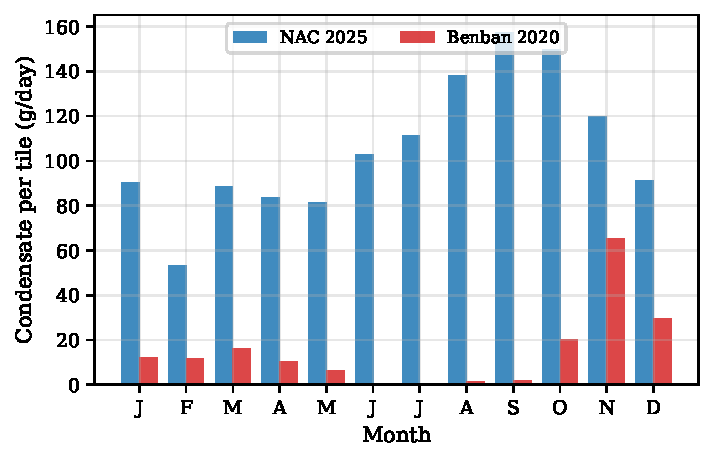
\includegraphics[width=0.72\textwidth]{figures/nac_monthly_water.pdf}
\caption{Monthly per-tile condensate, NAC 2025 against Benban 2020. The
Benban profile collapses in summer (June--September dew points sit below
the frost-protected plate floor most nights); the NAC profile peaks in
exactly those months.}
\label{fig:monthly}
\end{figure}

% =============================================================================
\section{Residential array assumptions}
\label{sec:array}
% =============================================================================

Table~\ref{tab:array} states every assumption behind the host array. The
\SIrange{3}{20}{\kWp} residential band is the project's own scale
definition; a villa or duplex roof near the top of that band is taken as
the reference. The soiling rate uses the mid-point of the
\SIrange{0.3}{0.8}{\percent\per\dy} arid-site band already cited in the
corpus \cite{kazem2023soiling}: greater-Cairo urban desert combines
construction dust with traffic particulates, so the lower edge of the band
is not defensible, while the upper edge belongs to active dust corridors
like Benban. The \num{3.5}-day cleaning interval is the existing
soiling-economics result (every 3--4 days) carried over unchanged; weekly
cleaning appears in Section~\ref{sec:awg} as a sensitivity row.

\begin{table}[ht]
\centering
\caption{Residential reference array, New Administrative Capital.}
\label{tab:array}
\begin{tabular}{@{}llp{6.0cm}@{}}
\toprule
\textbf{Item} & \textbf{Value} & \textbf{Basis}\\
\midrule
Module & LONGi LR5-72HPH-550M & Hi-MO~5 datasheet family
  \cite{longi2022himo5}; same frame as the CAD reference module\\
Count / array power & 18 / \SI{9.9}{\kWp} & top of the residential
  \SIrange{3}{20}{\kWp} scale band in the project scope\\
Module area / array area & \SI{2.556}{\metre\squared} /
  \SI{46.0}{\metre\squared} & \qtyproduct{2256 x 1133}{\milli\metre}
  per datasheet\\
Tilt / azimuth & \ang{26} / south & latitude tilt at \ang{30}N rooftops,
  rounded to typical racking\\
Daily array output & \SI{45.2}{\kilo\watt\hour\per\dy} &
  \SI{9.9}{\kWp} $\times$ \SI{5.71}{\kilo\watt\hour\per\metre\squared\per\dy}
  $\times$ PR \num{0.80} \cite{nasa_power_nac2025}\\
Soiling rate & \SI{0.5}{\percent\per\dy} & mid-point of the arid-site
  \SIrange{0.3}{0.8}{\percent\per\dy} band \cite{kazem2023soiling}\\
Cleaning dose & \SI{0.3}{\liter\per\metre\squared} per event & microfibre
  brush plus light spray (\texttt{project\_inputs.yaml})\\
Water per event & \SI{13.8}{\liter} & dose $\times$ \SI{46.0}{\metre\squared}\\
Cleaning interval & \SI{3.5}{\dy} (\num{104} events/yr) & existing
  soiling-economics optimum, 3--4 day band\\
Annual cleaning demand & \SI{1439}{\liter\per\yr} & \num{104.3} events
  $\times$ \SI{13.8}{\liter}\\
\bottomrule
\end{tabular}
\end{table}

% =============================================================================
\section{Tile performance: NAC against Benban}
\label{sec:tile}
% =============================================================================

The simulation engine, its psychrometrics, the TEC1-12706 coefficients
\cite{tec12706ds}, the \SI{5}{\kelvin} sub-cooling margin, and the smart
night-only strategy are all unchanged; only the climate file and site
pressure differ. Table~\ref{tab:compare} sets the two sites side by side.

\begin{table}[ht]
\centering
\caption{Per-tile annual performance, identical model and strategy.}
\label{tab:compare}
\begin{tabular}{@{}lS[table-format=4.2]S[table-format=4.2]l@{}}
\toprule
\textbf{Quantity} & {\textbf{Benban 2020}} & {\textbf{NAC 2025}} &
\textbf{Ratio / note}\\
\midrule
Water yield (\si{\liter\per\yr})        & 5.35  & 38.68 & 7.2$\times$\\
Water yield (\si{\gram\per\dy})         & 14.7  & 106.0 & 7.2$\times$\\
Electrical energy (\si{\kilo\watt\hour\per\yr}) & 22.25 & 56.03 &
  2.5$\times$ (more useful hours)\\
SEC, thermodynamic (\si{\kilo\watt\hour\per\liter}) & 4.16 & 1.45 &
  2.9$\times$ better\\
Mean operating COP                       & 1.44  & 1.91  & higher dew points\\
Operating hours per year                 & {---} & 3610  &
  \SI{9.9}{\hour} per night average\\
Best month (\si{\gram\per\dy})  & 65.4 & 157.2 & {Nov / Sep}\\
Worst month (\si{\gram\per\dy}) & 0.0  & 53.2  & {Jul (off) / Feb}\\
\bottomrule
\end{tabular}
\end{table}

Two findings matter for the thesis. First, the NAC profile has no dead
season: the worst month still delivers half the annual mean, whereas Benban
shuts down for most of June through September. Second, the specific energy
consumption falls below \SI{1.5}{\kilo\watt\hour\per\liter}
(thermodynamic), which moves the TEC approach from the pessimistic end of
the literature band into its mid-range. The Benban run keeps its role as
the worst-case feasibility floor.

% =============================================================================
\section{Dockside AWG sizing: the honest water balance}
\label{sec:awg}
% =============================================================================

\subsection{Why full self-supply is now feasible}

An earlier draft used a wet-wash dose of \SI{1.8}{\liter\per\metre\squared},
which made full self-supply impractical: it needed roughly 224 tiles drawing
about \SI{38}{\kilo\watt\hour\per\dy}, around \SI{84}{\percent} of array
output. That figure was the wet-wash worst case. The robot cleans with a
microfibre brush and a light spray, so the dose is
\SI{0.3}{\liter\per\metre\squared}, a sixfold cut that drops the demand to
\SI{1439}{\liter\per\yr}. At \SI{38.68}{\liter\per\yr} per tile, full
atmospheric self-supply needs 38 tiles drawing
\SI{6.47}{\kilo\watt\hour\per\dy} with fans, which is \SI{14}{\percent} of
the \SI{45.2}{\kilo\watt\hour\per\dy} the host array produces. On a weekly
cleaning schedule the demand halves to \SI{720}{\liter\per\yr}, met by 19
tiles at \SI{3.25}{\kilo\watt\hour\per\dy}, about \SI{7}{\percent} of array
output. Full closure is now the design target rather than an aspiration.

\subsection{Self-supply fraction trade}

Table~\ref{tab:trade} prices the dock at three self-supply fractions and
two cleaning frequencies, using the frozen sizing method (night harvest
from battery, dedicated PV recharge, \SI{20}{\percent} battery margin) and
the unit prices of the market BOM.

\begin{table}[ht]
\centering
\caption{Dock AWG trade study. Energy is the dock total (TEC + fans +
controller); cost is the standalone off-grid \texttt{dock\_total} (dedicated
PV + battery) at MARKET\_BOM unit prices (EGP, June 2026).}
\label{tab:trade}
\begin{tabular}{@{}lS[table-format=3.0]S[table-format=2.2]S[table-format=4.0]S[table-format=4.0]S[table-format=6.0]@{}}
\toprule
\textbf{Case} & {\textbf{Tiles}} & {\textbf{kWh/d}} & {\textbf{PV (Wp)}} &
{\textbf{Batt.\ (Ah)}} & {\textbf{Dock (EGP)}}\\
\midrule
\multicolumn{6}{@{}l}{\emph{Cleaning every \SI{3.5}{\dy} (demand \SI{1439}{\liter\per\yr})}}\\
$f=0.25$            & 10 & 1.75 &  383 &  228 &  85320\\
$f=0.50$            & 19 & 3.25 &  712 &  426 & 137253\\
$f=1.00$ (selected) & 38 & 6.47 & 1416 &  849 & 224756\\
\multicolumn{6}{@{}l}{\emph{Weekly cleaning (demand \SI{720}{\liter\per\yr}, sensitivity)}}\\
$f=0.25$            &  5 & 0.92 &  202 &  119 &  51735\\
$f=0.50$            & 10 & 1.75 &  383 &  228 &  85320\\
$f=1.00$            & 19 & 3.25 &  712 &  426 & 137253\\
\bottomrule
\end{tabular}
\end{table}

The selected point is $f=1.00$ at the \num{3.5}-day interval: 38 tiles
deliver the full \SI{1439}{\liter\per\yr} for \SI{6.47}{\kilo\watt\hour\per\dy},
which is \SI{14}{\percent} of the array's daily output. The weekly schedule
reaches full closure with 19 tiles at \SI{3.25}{\kilo\watt\hour\per\dy},
about \SI{7}{\percent} of array output, and is the cheaper alternative when
the soiling economics allow a longer interval. The standalone
\texttt{dock\_total} figures above include the dock's own dedicated off-grid
PV and battery, which dominate the cost; the marginal AWG hardware for the
38-tile stack (tiles, heat sinks, fans, cold plate, switching) is about
\num{14000}~EGP when the dock draws from the house array instead. The case
for the AWG is water quality, autonomy, and now full self-supply: condensate
is distilled, leaves no scale film on the glass, and keeps the robot
operational through mains interruptions.

\subsection{Selected dock configuration}

\begin{itemize}[nosep]
  \item \textbf{AWG stack:} 38 $\times$ TEC1-12706 \cite{futelec2026tec},
        extruded fin section, 20 axial fans, cold plates and switching;
        about \num{14000}~EGP for the marginal hardware.
  \item \textbf{Supply (grid-coupled, recommended):} the dock sits beside a
        net-metered house with its own \SI{9.9}{\kWp} array, so it draws its
        \SI{6.47}{\kilo\watt\hour} night load from the house bus through a
        \SI{500}{\watt}-class \SI{12}{\volt} supply and needs no dedicated
        PV, MPPT, or bank. The marginal AWG hardware is then about
        \num{14000}~EGP.
  \item \textbf{Supply (standalone option, priced):} \SI{1416}{\Wp} required,
        met by 3~$\times$ Jinko \SI{580}{\Wp} \cite{jinko2024tigerneo}; EPever
        \SI{60}{\ampere} MPPT \cite{epever2023tracer}; \SI{849}{\ampere\hour}
        battery requirement met by 5~$\times$ \SI{200}{\ampere\hour}
        LiFePO$_4$ packs. This dedicated supply dominates the
        \num{224756}~EGP standalone \texttt{dock\_total}; it is priced only
        because the frozen sizing method is off-grid.
  \item \textbf{Tanks:} \SI{300}{\liter} HDPE storage tank to bridge seasonal
        yield swings (the worst month delivers about half the annual mean),
        feeding the distilled AWG output to the robot. Local supply, about
        \num{3000}~EGP with plumbing.
\end{itemize}

At \SI{3.94}{\liter\per\dy} the AWG fills one whole-array cleaning charge
over each \num{3.5}-day interval: \SI{3.94}{\liter\per\dy} accumulates the
full \SI{13.8}{\liter} event charge between cleanings, so the AWG supplies
every event directly with no mains top-up. The \SI{300}{\liter} tank holds
the surplus from high-yield months against the leaner ones.

% =============================================================================
\section{Robot compatibility check}
\label{sec:robot}
% =============================================================================

The robot is mechanically unchanged. Three checks follow from the new
host array.

\paragraph{Tilt.} The CAD package fixes the design basis at \ang{24}
panel tilt; the NAC racking is \ang{26}. Recomputing the frozen traction
model at \ang{26} gives a resistive force of \SI{33.7}{\newton}
(\SI{32.0}{\newton} at \ang{24}, a \SI{5.4}{\percent} rise) and
\SI{0.723}{\newton\metre} per motor through the \num{0.7}-efficient
drivetrain. With the 1.5 design factor the demand is
\SI{1.084}{\newton\metre}, still inside the Pololu \#4756 continuous band
of \SI{1.108}{\newton\metre} \cite{pololu4756}, with a
\SI{4.1}{$\times$} stall margin. The check passes, but the continuous-band
headroom at the factored demand is only \SI{2}{\percent}, so the CAD
design-basis note (D-107, ``tilted up to \ang{24}'') should be revised to
\ang{26} and the traction table updated. The \ang{15} condensate drain
tilt on the dock is unaffected.

\paragraph{Coverage route.} Per module
(\qtyproduct{2256 x 1133}{\milli\metre}, portrait), the
\SI{225}{\milli\metre} effective brush width gives 6 boustrophedon passes,
a \SI{14.7}{\metre} path, and \SI{308}{\second} including turns. A full
event over 18 modules is \SI{264}{\metre} of sweeping, about
\SI{92}{\minute} plus transfers, and \SI{74}{\watt\hour} of drive and pump
energy. Transfers between modules that share a mounting plane and flush
frames are driven directly; transfers between separated rows are not
within the crawler's capability and need either a transfer ramp at the row
ends or manual repositioning. The residential reference layout therefore
assumes the common villa pattern of one or two contiguous racking planes.

\paragraph{Water per module.} At the \SI{0.3}{\liter\per\metre\squared}
microfibre dose the cleaning charge is \SI{0.6}{\liter} for a
\SI{2.0}{\metre\squared} panel; the \SI{2.556}{\metre\squared} residential
module needs \SI{0.77}{\liter} per pass. Both fit the onboard tank inside
the \qtyproduct{460 x 300 x 155}{\milli\metre} envelope with margin, so the
tank stretch flagged under the old wet-wash dose is no longer needed and the
robot does not have to dock mid-event to refill.

% =============================================================================
\section{Bill-of-materials delta}
\label{sec:bom}
% =============================================================================

Table~\ref{tab:bom} restates the market BOM full-scale rollup for the
recommended NAC residential design, at the same unit prices and the same
\num{48}~EGP/USD basis. Two supply cases are shown: the standalone off-grid
dock with its own PV and battery, and the grid-coupled dock that draws its
night load from the house array.

\begin{table}[ht]
\centering
\caption{Full-system cost, NAC residential 100\,\% self-supply (38 tiles),
standalone against grid-coupled supply (EGP, June 2026 unit prices).}
\label{tab:bom}
\begin{tabular}{@{}p{6.4cm}S[table-format=6.0]S[table-format=6.0]S[table-format=-6.0]@{}}
\toprule
\textbf{Subsystem} & {\textbf{Standalone}} & {\textbf{Grid-coupled}} &
{\textbf{Delta}}\\
\midrule
AWG stack (tiles, fins, fans, plates, switching) & 13756 & 13756 & 0\\
Dedicated supply (PV, MPPT, battery bank) & 211000 & 0 & -211000\\
Mobility and cleaning (unchanged robot) & 16220 & 16220 & 0\\
Control and sensing (unchanged) & 7970 & 7970 & 0\\
Storage tank and plumbing & 3000 & 3000 & 0\\
\midrule
\textbf{Total} & 251946 & 40946 & -211000\\
\bottomrule
\end{tabular}
\end{table}

The dedicated off-grid supply dominates the standalone cost: the dock's own
PV, MPPT, and battery bank account for \num{211000} of the
\num{251946}~EGP total. Because the house already carries a
\SI{9.9}{\kWp} array, the grid-coupled dock deletes that supply and the
marginal AWG hardware for full self-supply is about \num{14000}~EGP, so the
grid-coupled configuration is the recommended choice for any roof with a
net-metered connection.

% =============================================================================
\section{Conclusion: what changes in the thesis}
% =============================================================================

The reference deployment case moves from a utility-scale panel at Benban
to an 18-module, \SI{9.9}{\kWp} residential rooftop in the New
Administrative Capital, simulated on NASA POWER 2025 hourly data
\cite{nasa_power_nac2025}. The Benban chapter is retained unchanged as
feasibility evidence: it proves the TEC tile condenses water in the
worst Egyptian climate the robot will meet. The NAC run then carries the
design numbers: \SI{38.7}{\liter\per\yr} per tile at a mean COP of
\num{1.91}, and, with the microfibre robot's \SI{0.3}{\liter\per\metre\squared}
dose cutting demand to \SI{1.44}{\cubic\metre\per\yr}, full atmospheric
self-supply is feasible at 38 tiles drawing \SI{14}{\percent} of array
energy (19 tiles and \SI{7}{\percent} on a weekly schedule). A
\SI{300}{\liter} storage tank bridges the seasonal yield swing, and the
grid-tied AWG hardware costs about \num{14000}~EGP because the house array
carries the night load. The \SI{1.8}{\liter\per\metre\squared} wet-wash
figure of the earlier draft was revised to the robot's actual low-water
cleaning. The robot hardware survives the move with one flagged revision,
the \ang{26} tilt note, and one stated limitation, single-plane transfers
only. The thesis should also carry the New Alamein sensitivity run, where
coastal humidity will raise per-tile yield further; that is the natural
next computation with the same script and a new coordinate pair.

\bibliographystyle{ieeetr}
\bibliography{references}

\end{document}
